\documentclass[dvipdfmx,11pt]{beamer}

%全体設定
%\AtBeginDvi{\special{pdf:tounicode 90ms-RKSJ-UCS2}}

\usepackage{bxdpx-beamer}% dvipdfmxなので必要
\usepackage{pxjahyper}
\usepackage{minijs}
\usepackage{otf}
\usepackage{amssymb,amsmath}
\usepackage{hyperref}
\usepackage[absolute,overlay]{textpos}
\usepackage{comment}
\usepackage{colortbl}
\usepackage{graphicx}
\usepackage{tikz}
\usetikzlibrary{positioning}
\usetikzlibrary{shadows}
\usepackage{listings}
\usepackage{plistings}
\def\lstlistingname{コード}

\renewcommand{\kanjifamilydefault}{\gtdefault}
%%\usetheme{Frankfurt}
\usetheme{Warsaw}
\setbeamertemplate{navigation symbols}{} %スライドのボタン?(右下のやつ)を消す
\setbeamersize{text margin left=1.5em,text margin right=1.5em} % 余白なくすやつ

\title{解集合プログラミングを用いた\\配電網問題の解法に関する考察}
\author{山田 健太郎}
\date{卒業研究発表会\\2020年2月20日}
\institute{番原研究室}

%% テンプレ 
\begin{comment}

%%%%%%%%%%%%%%%%%%%%%%%%%%%%%%%%%%%%%%%%%%%%%%%%%%
%% タイトル
%%%%%%%%%%%%%%%%%%%%%%%%%%%%%%%%%%%%%%%%%%%%%%%%%%
\begin{frame}\frametitle{}
\end{frame}

\end{comment}

%###########################################################
%# 本文 ####################################################
%###########################################################
\begin{document}

%%%%%%%%%%%%%%%%%%%%%%%%%%%%%%%%%%%%%%%%%%%%%%%%%%
%% タイトル 
%%%%%%%%%%%%%%%%%%%%%%%%%%%%%%%%%%%%%%%%%%%%%%%%%%
\begin{frame}\frametitle{}
  \titlepage
\end{frame}

%%%%%%%%%%%%%%%%%%%%%%%%%%%%%%%%%%%%%%%%%%%%%%%%%%
% 配電網
%%%%%%%%%%%%%%%%%%%%%%%%%%%%%%%%%%%%%%%%%%%%%%%%%%
\begin{frame}\frametitle{配電網問題}
 \begin{alertblock}{}
  \centering
  求解困難な組合せ最適化問題の一種
 \end{alertblock}

 \begin{itemize}
  \item  \alert{配電網}とは,変電所と,家庭や工場などから構成される
		 電力供給経路のネットワークである.
  \item  配電網の構成技術はスマートグリッドや,災害時の障害箇所の迂回構成などを支える
		 重要な基盤技術として期待されている.
  \item  \alert{配電網問題}とは,
		 \begin{itemize}
		  \item \structure{トポロジ制約}と\structure{電気制約}から構成.
		  \item 損失電力を最小にするスイッチの開閉状態を求めることが目的.
		 \end{itemize}
  \item フロンティア法を用いた解法が提案されている[井上ほか '12]. 
		\begin{itemize}
		 \item ERATO湊離散構造処理系プロジェクトの成果.
		 \item 実用規模の配電網問題(\structure{\textbf{スイッチ数468個}})の最適解を発見.
		\end{itemize}
 \end{itemize}

 \vspace{-0.25cm}
 \pause
 \begin{alertblock}{}
  トポロジ制約のみの配電網問題は,グラフと根と呼ばれる特別なノードから,
  \alert{根付き全域森}を求める部分グラフ探索問題に帰着できる.
 \end{alertblock}
  
\end{frame}

%%%%%%%%%%%%%%%%%%%%%%%%%%%%%%%%%%%%%%%%%%%%%%%%%%
%% 根付き全域森
%%%%%%%%%%%%%%%%%%%%%%%%%%%%%%%%%%%%%%%%%%%%%%%%%%
\begin{frame}\frametitle{根付き全域森(Spanning Rooted Forest)}

 \begin{block}{根付き全域森~~[川原$\cdot$湊 '12]}
  グラフ$G=(V,E)$と,
  \alert{根}と呼ばれる$V$上のノードが与えられたとき,
  $G$上の根付き全域森とは,以下の条件を満たす$G$の部分グラフ$G'=(V,E'),\ E' \subseteq E$である.
  \begin{enumerate}
   \item $G'$はサイクルを持たない. (\alert{非閉路制約})
   \item $G'$の各連結成分は,ちょうど1つの根を含む. (\alert{根付き連結制約})
  \end{enumerate}
 \end{block}

 \begin{exampleblock}{根付き全域森の例}
  \begin{columns}
   \begin{column}{0.45\textwidth}
	\centering
	%%%%%%%%%%%%%%%%%%%%%%%%%%%%%%%%%%%%%%%%%%%%%%%%%%
% 根付き全域森の例
%%%%%%%%%%%%%%%%%%%%%%%%%%%%%%%%%%%%%%%%%%%%%%%%%%

\begin{tikzpicture}[scale=0.5]

 % 設定
 \tikzset{node/.style={circle,draw=black,fill=white}}

 \definecolor{edge1}{RGB}{191,0,0}
 \definecolor{node1}{RGB}{249,200,200}
 \definecolor{edge3}{RGB}{38,38,134}
 \definecolor{node3}{RGB}{200,200,249}

 % 補助線
 % \draw [help lines,blue] (0,0) grid (20,6);

 % 入力されるグラフ
 % node %
 \node[circle, ultra thick,draw=edge1,fill=node1] (in1) {1};
 \node[node,right= of in1] (in2){2};
 \node[circle, ultra thick, draw=edge3,fill=node3, right=of in2](in3){3};
 \node[node,below= of in1] (in4){4};
 \node[node,below= of in2] (in5){5};
 \node[node,below= of in3] (in6){6};

 % 辺
 \foreach \u / \v in {in1/in2,in2/in3,in1/in4,in2/in5,in3/in6,in4/in5,in5/in6}
 \draw (\u) -- (\v);

\end{tikzpicture}

%%%%%%%%%%%%%%%%%%%%%%%%%%%%%%%%%%%%%%%%%%%%%%%%%%%%%%%%%%
%%% Local Variables:
%%% mode: japanese-latex
%%% TeX-master: ``slide''
%%% End:

   \end{column}
   \begin{column}{0.45\textwidth}
	\centering
	%%%%%%%%%%%%%%%%%%%%%%%%%%%%%%%%%%%%%%%%%%%%%%%%%%
% 根付き全域森の例
%%%%%%%%%%%%%%%%%%%%%%%%%%%%%%%%%%%%%%%%%%%%%%%%%%

\begin{tikzpicture}[scale=0.5]

 % 設定
 \tikzset{node/.style={circle,draw=black,fill=white}}

 \definecolor{edge1}{RGB}{191,0,0}
 \definecolor{node1}{RGB}{249,200,200}
 \definecolor{edge3}{RGB}{38,38,134}
 \definecolor{node3}{RGB}{200,200,249}

 % 補助線
 % \draw [help lines,blue] (0,0) grid (20,6);

 % node %
 \node[circle, ultra thick, draw=edge1, fill=node1](out1){1};
 \node[node, fill=node1, right=of out1] (out2){2};
 \node[circle, ultra thick, draw=edge3,fill=node3, right=of out2](out3){3};
 \node[node, fill=node1, below=of out1] (out4){4};
 \node[node, fill=node3, below=of out2] (out5){5};
 \node[node, fill=node3, below=of out3] (out6){6};

 \foreach \u / \v in {out1/out2,out1/out4}
 \draw [very thick, edge1] (\u) -- (\v);

 \foreach \u / \v in {out3/out6,out5/out6}
 \draw [very thick, edge3](\u) -- (\v);

\end{tikzpicture}

%%%%%%%%%%%%%%%%%%%%%%%%%%%%%%%%%%%%%%%%%%%%%%%%%%%%%%%%%%
%%% Local Variables:
%%% mode: japanese-latex
%%% TeX-master: ``slide''
%%% End:

   \end{column}
  \end{columns}


 \end{exampleblock}
 
\end{frame}

%%%%%%%%%%%%%%%%%%%%%%%%%%%%%%%%%%%%%%%%%%%%%%%%%%
%% ASP
%%%%%%%%%%%%%%%%%%%%%%%%%%%%%%%%%%%%%%%%%%%%%%%%%%
\begin{frame}\frametitle{解集合プログラミング(Answer Set Programming; ASP)}
 \begin{itemize}
  \item \structure{ASP言語}は一階論理に基づく知識表現言語の一種である.
  \item \structure{ASPシステム}は論理プログラムから安定モデル意味論[Gelfond and Lifschitz '88]に
		基づく解集合を計算するシステムである.
  \item 近年ではSAT技術を応用した高速ASPシステムが実現され,システム検証,プランニング,
		システム生物学など様々な分野への応用が拡大している.
 \end{itemize}

 \begin{alertblock}{ASP技術を組合せ最適化問題に用いる利点}
   \begin{itemize}
	\item ASP言語の高い表現力を活かし,記号的な制約を簡潔に記述可能.
	\item ASPMT技術を用いて,様々な背景理論ソルバーと連携可能.
	\item 充足不能コアを用いた効率的な最適値探索が利用可能.
%	\item ASPシステムの持つ高い拡張性により,新たな制約の追加が容易.
   \end{itemize}
 \end{alertblock}

\end{frame}

%%%%%%%%%%%%%%%%%%%%%%%%%%%%%%%%%%%%%%%%%%%%%%%%%%
%% 研究目的
%%%%%%%%%%%%%%%%%%%%%%%%%%%%%%%%%%%%%%%%%%%%%%%%%%
\begin{frame}\frametitle{研究目的}
 \begin{alertblock}{目的}
  % \centering
  ASP技術を活用して,大規模な配電網問題を効率良く解くシステムの\\構築を目指す.
 \end{alertblock}

 \begin{block}{研究内容}
  \begin{enumerate}
   \item \structure{根付き全域森問題を解く,2種類のASP符号化を考案した.}
   % \begin{itemize}
   % 	\item 上限,下限に基づく符号化.
   % 	\item ASP言語の表現性を利用した符号化.
	 % \end{itemize}
   \item \structure{実用規模の問題,及び,より大規模な問題を用いた評価実験.}
   % \begin{itemize}
   % 	\item 問題の規模に関する比較評価.
   % 	\item 生成される制約の数の比較評価.
   % \end{itemize
   \item 遷移問題へ拡張し,その符号化を考案した.
   \begin{itemize}
	\item ある配電網の構成(初期状態)から,目的とする配電網の構成(目的状態)を得るための,
		  スイッチの切替手順を求める問題.
   \end{itemize}
  \end{enumerate}
  
 \end{block}
 
\end{frame}

\begin{frame}\frametitle{ASPを用いた根付き全域森問題の解法}
 
 \begin{figure}[htbp]
  \centering
  %%%%%%%%%%%%%%%%%%%%%%%%%%%%%%%%%%%%%%%%%%%%%%%%%%
%% ASPで問題を解く流れの図
%%%%%%%%%%%%%%%%%%%%%%%%%%%%%%%%%%%%%%%%%%%%%%%%%%
\begin{tikzpicture}

 \definecolor{edge}{RGB}{38,38,134}
 \definecolor{node}{RGB}{220,220,249}

 \definecolor{alert_edge}{RGB}{191,0,0}
 \definecolor{alert_node}{RGB}{249,200,200}

 \def\nodehspace{1.5cm}

 \tikzset{block/.style={rectangle, thick, draw=edge, fill=node, text centered, 
 rounded corners, text width=1.5cm, minimum height=1.6cm,minimum width=1.5cm}};

 \tikzset{alertblock/.style={rectangle, thick, draw=alert_edge, fill=alert_node, 
 text centered, rounded corners, text width=1.5cm, minimum height=1.6cm}};

 \node[block](ins){HCP\\HPP};
 \node[block, right=\nodehspace of ins] (fact){ASP\\ファクト};
 \node[alertblock, below=of fact](encode){ASP\\符号化};
 \node[block, right=\nodehspace of fact](sys){ASP\\システム};
 \node[block, right=\nodehspace of sys] (ans){問題の解};

 \foreach \u / \v / \name in {ins/fact/変換,fact/sys/,encode/sys/,sys/ans/}
 \draw [thick,->] (\u) to node[above]{\name} (\v);

\end{tikzpicture}

 \end{figure}

 \vspace{-0.5cm}
 \begin{exampleblock}{}
  \begin{enumerate}
   \item 与えられた問題インスタンスをASPのファクト形式に変換する.
   \item 変換した問題と,根付き全域森問題を解くASP符号化を結合し,
		 ASPシステムを用いて解を求める.
  \end{enumerate}
 \end{exampleblock}
\end{frame}

%%%%%%%%%%%%%%%%%%%%%%%%%%%%%%%%%%%%%%%%%%%%%%%%%%
%% 提案手法
%%%%%%%%%%%%%%%%%%%%%%%%%%%%%%%%%%%%%%%%%%%%%%%%%%
\begin{frame}\frametitle{提案するASP符号化}
 
\begin{itemize}
 \item  根付き全域森問題に対する,2種類のASP符号化を考案した.
 \item $|V|$はグラフのノード数,$|R|$は根ノード数をそれぞれ表す.
\end{itemize}
 
\begin{table}[t]
 \centering
 %%%%%%%%%%%%%%%%%%%%%%%%%%%%%%%%%%%%%%%%%%%%%%%%%%%%%%%%%%
\chapter{クイーングラフ彩色問題のSMT符号化と$distinct$制約の高速化}
%%%%%%%%%%%%%%%%%%%%%%%%%%%%%%%%%%%%%%%%%%%%%%%%%%%%%%%%%%

本章ではSMTソルバーにおける$distinct$制約の高速化のために用いた手法についてそれぞれ述べる.
まず最初に,クイーングラフ彩色問題のSMT符号化について示し,次に高速化手法についてクイーングラフ彩色問題においてどのように表されるかを交えて説明を行う.

%%%%%%%%%%%%%%%%%%%%%%%%%%%%%%%%%%%%%%%%%%%%%%%%%%%%%%%%%%
%%
%% クイーングラフ彩色問題のSMT符号化
%%
%%%%%%%%%%%%%%%%%%%%%%%%%%%%%%%%%%%%%%%%%%%%%%%%%%%%%%%%%%
\section{クイーングラフ彩色問題のSMT符号化}
ここではN=5の場合のクイーングラフ彩色問題について使用したSMT符号化について説明する.
本研究ではチェス盤上の一番上の行を0行目,一番左の列を0列目とし,クイーンの色は整数として0から数えるものとする.


%%%%%%%%%%%%%%%%%%%%%%%%%%%%%%%%%%%%%%%%%%%%%%%%%%%%%%%%%%
\subsection{色変数モデルのSMT符号化}
%%%%%%%%%%%%%%%%%%%%%%%%%%%%%%%%%%%%%%%%%%%%%%%%%%%%%%%%%%
まず,整数変数c\_0\_0は以下のように宣言される.
c\_i\_jはi行j列目のクイーンの色を示している.
{ \scriptsize \begin{verbatim}
    (declare-const c_0_0 Int)
\end{verbatim}}
また,c\_0\_0は0以上4以下であるので以下の制約を追加する.
{ \scriptsize \begin{verbatim}
    (assert (and (>= c_0_0 0) (<= c_0_0 4)))
\end{verbatim}}
他の変数についても同様に宣言される.

次に,0行目に配置されるクイーンの色が互いに異なるという制約は以下のように宣言される.
{ \scriptsize \begin{verbatim}
    (assert (distinct c_0_0 c_0_1 c_0_2 c_0_3 c_0_4)))
\end{verbatim}}
他の行や列,右上がり対角線や右下がり対角線についても同様に宣言される.


作成したN=5の場合の色変数モデルのコードをコード\ref{code:qgcp_5_col}に示す.
3から52行目が各整数変数の宣言とそのドメインを指定しており,
53から57行目が各行についての制約であり,
58から62行目が各列について,
63から69行目が各右上がり対角線について,
70から76行目が角右下がり対角線についてである.
また,77から81行目は対称性除去のために0行目の値を指定している.

\lstinputlisting[float=htbp,caption={%
N=5の色変数モデルのクイーングラフ彩色問題},%
captionpos=b,frame=single,label=code:qgcp_5_col,%
numbers=left,%
breaklines=true,%
columns=fullflexible,keepspaces=true,%
basicstyle=\ttfamily\tiny]{code/qgcp_5_m0__z3_489.smt2}


%%%%%%%%%%%%%%%%%%%%%%%%%%%%%%%%%%%%%%%%%%%%%%%%%%%%%%%%%%
\subsection{位置変数モデルのSMT符号化}
%%%%%%%%%%%%%%%%%%%%%%%%%%%%%%%%%%%%%%%%%%%%%%%%%%%%%%%%%%
まず,整数変数y\_0\_0は以下のように宣言される.
y\_i\_kはi行目のk色のクイーンが配置される場所を示している.
{ \scriptsize \begin{verbatim}
    (declare-const y_0_0 Int)
\end{verbatim}}
また,y\_0\_0は0以上4以下であるので以下の制約を追加する.
{ \scriptsize \begin{verbatim}
    (assert (and (>= y_0_0 0) (<= y_0_0 4)))
\end{verbatim}}
他の変数についても同様に宣言される.

次に,0行目に配置される5色のクイーンがそれぞれ異なる列に配置されるという制約は以下のように宣言される.
{ \scriptsize \begin{verbatim}
    (assert (distinct y_0_0 y_0_1 y_0_2 y_0_3 y_0_4)))
\end{verbatim}}
他の行や列についても同様に宣言される.

右上がり対角線について,色0が配置される行と列の和が2つ以上同じにならないという制約は以下のように宣言される.
{ \scriptsize \begin{verbatim}
    (assert (distinct (+ y_0_0 0) (+ y_1_0 1) (+ y_2_0 2) (+ y_3_0 3) (+ y_4_0 4)))
\end{verbatim}}
他の色についても同様に宣言される.

右下がり対角線について,色0が配置される行と列の差が2つ以上同じにならないという制約は以下のように宣言される.
{ \scriptsize \begin{verbatim}
    (assert (distinct (- y_0_0 0) (- y_1_0 1) (- y_2_0 2) (- y_3_0 3) (- y_4_0 4)))
\end{verbatim}}
他の色についても同様に宣言される.


作成したN=5の場合の位置変数モデルのコードを\ref{code:qgcp_5_pos}に示す.
色変数モデルの時と同様にして,
3から52行目が各整数変数の宣言とそのドメインを指定しており,
53から72行目が各行,各列,各右上がり対角線,各右下がり対角線についてそれぞれ互いに異なるという制約を追加している.
また,73から77行目は対称性除去のために0行目に配置されるクイーンの列を指定して宣言している.

\lstinputlisting[float=htbp,caption={%
N=5の位置変数モデルのクイーングラフ彩色問題},%
captionpos=b,frame=single,label=code:qgcp_5_pos,%
numbers=left,%
breaklines=true,%
columns=fullflexible,keepspaces=true,%
basicstyle=\ttfamily\tiny]{code/qgcp_5_m7__z3_489.smt2}


%%%%%%%%%%%%%%%%%%%%%%%%%%%%%%%%%%%%%%%%%%%%%%%%%%%%%%%%%%
\subsection{0-1変数モデルのSMT符号化}\label{sec:pro_pb}
%%%%%%%%%%%%%%%%%%%%%%%%%%%%%%%%%%%%%%%%%%%%%%%%%%%%%%%%%%

% 高速化のための2つ目の手法は$distinct$制約をPB符号化して解くというものである.
% この手法では,求める解を整数変数としてではなく0-1変数として求める.
%
% 例としては,整数変数$x \in \{1,2,3\}$は0-1変数$x_1,x_2,x_3 \in {0,1}$として,$x_i=1$なら$x=i$というようにして解を求める.
%
% N=5の場合について本研究で使用したSMT符号化を説明する
まず,0-1変数c\_0\_0\_0は以下のように宣言される.
c\_i\_j\_kはi行j列目がk色に塗られるかどうかを示している.
{ \scriptsize \begin{verbatim}
    (declare-const c_0_0_0 Int)
\end{verbatim}}
また,c\_0\_0\_0は0-1変数であるので以下の制約を追加する.
{ \scriptsize \begin{verbatim}
    (assert (and (>= c_0_0_0 0) (<= c_0_0_0 1)))
\end{verbatim}}
他の変数についても同様に宣言される.
盤面上の一つのマスに塗られる色は一色だけなので,0行0列目が一つの色で塗られる制約は以下のようになる.
{ \scriptsize \begin{verbatim}
(assert (= (+ c_0_0_0 c_0_0_1 c_0_0_2 c_0_0_3 c_0_0_4) 1))
\end{verbatim}}
他のマスについても同様に宣言される.この制約は式\ref{eq:smt_pb_1}に対応しており,重複を避けるためにまとめて宣言する.

次に,0行目に配置されるクイーンの色が互いに異なるという制約は以下のように宣言される.
{ \scriptsize \begin{verbatim}
(assert (= (+ c_0_0_0 c_0_1_0 c_0_2_0 c_0_3_0 c_0_4_0) 1))
(assert (= (+ c_0_0_1 c_0_1_1 c_0_2_1 c_0_3_1 c_0_4_1) 1))
(assert (= (+ c_0_0_2 c_0_1_2 c_0_2_2 c_0_3_2 c_0_4_2) 1))
(assert (= (+ c_0_0_3 c_0_1_3 c_0_2_3 c_0_3_3 c_0_4_3) 1))
(assert (= (+ c_0_0_4 c_0_1_4 c_0_2_4 c_0_3_4 c_0_4_4) 1))
\end{verbatim}}
他の行や列についても同様に宣言される.

右上がり対角線について,\verb|c_0_3, c_1_2, c_2_1, c_3_0|が互いに異なるという制約は以下のように宣言される.
{ \scriptsize \begin{verbatim}
(assert (<= (+ c_0_3_0 c_1_2_0 c_2_1_0 c_3_0_0) 1))
(assert (<= (+ c_0_3_1 c_1_2_1 c_2_1_1 c_3_0_1) 1))
(assert (<= (+ c_0_3_2 c_1_2_2 c_2_1_2 c_3_0_2) 1))
(assert (<= (+ c_0_3_3 c_1_2_3 c_2_1_3 c_3_0_3) 1))
(assert (<= (+ c_0_3_4 c_1_2_4 c_2_1_4 c_3_0_4) 1))
\end{verbatim}}
他の右上がり対角線についても同様に宣言されるが,$i+j=N-1$の場合は上記の\verb|<=|は\verb|=|に変更して以下のように宣言される.
{ \scriptsize \begin{verbatim}
(assert (= (+ c_0_4_0 c_1_3_0 c_2_2_0 c_3_1_0 c_4_0_0) 1))
(assert (= (+ c_0_4_1 c_1_3_1 c_2_2_1 c_3_1_1 c_4_0_1) 1))
(assert (= (+ c_0_4_2 c_1_3_2 c_2_2_2 c_3_1_2 c_4_0_2) 1))
(assert (= (+ c_0_4_3 c_1_3_3 c_2_2_3 c_3_1_3 c_4_0_3) 1))
(assert (= (+ c_0_4_4 c_1_3_4 c_2_2_4 c_3_1_4 c_4_0_4) 1))
\end{verbatim}}
右下がり対角線については$i-j=N-1$の場合に\verb|<=|を\verb|=|に変更し同様にして宣言される.


作成したN=5の場合の色変数モデルのコードをコード\ref{code:qgcp_5_pb}に示す.
3から277行目が各整数変数の宣言とそのドメインと色の制約を追加しており,
278から425行目が各行,各列,各右上がり対角線,各右下がり対角線についてそれぞれ互いに異なるという制約を追加している.
また,426から430行目は対称性除去のために0行目の値を指定している.

\begin{lstlisting}[frame=trl,numbers=left,breaklines=true,%
columns=fullflexible,keepspaces=true,%
basicstyle=\ttfamily\scriptsize]
; QGCP model=18 n=5 opts={'-m': '18', '-x': ''}
; color-variable model (pb)
(declare-const c_0_0_0 Int)
(assert (and (>= c_0_0_0 0) (<= c_0_0_0 1)))
(declare-const c_0_0_1 Int)
(assert (and (>= c_0_0_1 0) (<= c_0_0_1 1)))
(declare-const c_0_0_2 Int)
(assert (and (>= c_0_0_2 0) (<= c_0_0_2 1)))
(declare-const c_0_0_3 Int)
(assert (and (>= c_0_0_3 0) (<= c_0_0_3 1)))
(declare-const c_0_0_4 Int)
(assert (and (>= c_0_0_4 0) (<= c_0_0_4 1)))
(declare-const c_0_1_0 Int)
(assert (and (>= c_0_1_0 0) (<= c_0_1_0 1)))
(declare-const c_0_1_1 Int)
(assert (and (>= c_0_1_1 0) (<= c_0_1_1 1)))
(declare-const c_0_1_2 Int)
(assert (and (>= c_0_1_2 0) (<= c_0_1_2 1)))
(declare-const c_0_1_3 Int)
(assert (and (>= c_0_1_3 0) (<= c_0_1_3 1)))
(declare-const c_0_1_4 Int)
(assert (and (>= c_0_1_4 0) (<= c_0_1_4 1)))
(declare-const c_0_2_0 Int)
(assert (and (>= c_0_2_0 0) (<= c_0_2_0 1)))
(declare-const c_0_2_1 Int)
(assert (and (>= c_0_2_1 0) (<= c_0_2_1 1)))
(declare-const c_0_2_2 Int)
(assert (and (>= c_0_2_2 0) (<= c_0_2_2 1)))
(declare-const c_0_2_3 Int)
(assert (and (>= c_0_2_3 0) (<= c_0_2_3 1)))
(declare-const c_0_2_4 Int)
(assert (and (>= c_0_2_4 0) (<= c_0_2_4 1)))
(declare-const c_0_3_0 Int)
(assert (and (>= c_0_3_0 0) (<= c_0_3_0 1)))
(declare-const c_0_3_1 Int)
(assert (and (>= c_0_3_1 0) (<= c_0_3_1 1)))
(declare-const c_0_3_2 Int)
(assert (and (>= c_0_3_2 0) (<= c_0_3_2 1)))
(declare-const c_0_3_3 Int)
(assert (and (>= c_0_3_3 0) (<= c_0_3_3 1)))
(declare-const c_0_3_4 Int)
(assert (and (>= c_0_3_4 0) (<= c_0_3_4 1)))
(declare-const c_0_4_0 Int)
(assert (and (>= c_0_4_0 0) (<= c_0_4_0 1)))
(declare-const c_0_4_1 Int)
(assert (and (>= c_0_4_1 0) (<= c_0_4_1 1)))
(declare-const c_0_4_2 Int)
(assert (and (>= c_0_4_2 0) (<= c_0_4_2 1)))
(declare-const c_0_4_3 Int)
(assert (and (>= c_0_4_3 0) (<= c_0_4_3 1)))
(declare-const c_0_4_4 Int)
(assert (and (>= c_0_4_4 0) (<= c_0_4_4 1)))
\end{lstlisting}
$\vdots$
\begin{lstlisting}[frame=rl,numbers=left,breaklines=true,%
columns=fullflexible,keepspaces=true,%
basicstyle=\ttfamily\scriptsize,firstnumber=253]
(assert (= (+ c_0_0_0 c_0_0_1 c_0_0_2 c_0_0_3 c_0_0_4) 1))
(assert (= (+ c_0_1_0 c_0_1_1 c_0_1_2 c_0_1_3 c_0_1_4) 1))
(assert (= (+ c_0_2_0 c_0_2_1 c_0_2_2 c_0_2_3 c_0_2_4) 1))
(assert (= (+ c_0_3_0 c_0_3_1 c_0_3_2 c_0_3_3 c_0_3_4) 1))
(assert (= (+ c_0_4_0 c_0_4_1 c_0_4_2 c_0_4_3 c_0_4_4) 1))
\end{lstlisting}
$\vdots$

\begin{lstlisting}[frame=rl,numbers=left,breaklines=true,%
columns=fullflexible,keepspaces=true,%
basicstyle=\ttfamily\scriptsize,firstnumber=278]
; alldiff_pb c_0_0 c_0_1 c_0_2 c_0_3 c_0_4
(assert (= (+ c_0_0_0 c_0_1_0 c_0_2_0 c_0_3_0 c_0_4_0) 1))
(assert (= (+ c_0_0_1 c_0_1_1 c_0_2_1 c_0_3_1 c_0_4_1) 1))
(assert (= (+ c_0_0_2 c_0_1_2 c_0_2_2 c_0_3_2 c_0_4_2) 1))
(assert (= (+ c_0_0_3 c_0_1_3 c_0_2_3 c_0_3_3 c_0_4_3) 1))
(assert (= (+ c_0_0_4 c_0_1_4 c_0_2_4 c_0_3_4 c_0_4_4) 1))
\end{lstlisting}
$\vdots$

\begin{lstlisting}[frame=rbl,numbers=left,breaklines=true,%
columns=fullflexible,keepspaces=true,%
basicstyle=\ttfamily\scriptsize,firstnumber=426,%
captionpos=b,caption={N=5の0-1変数のみを用いた色変数モデルのクイーングラフ彩色問題},label={code:qgcp_5_pb}]
(assert (= c_0_0_0 1))
(assert (= c_0_1_1 1))
(assert (= c_0_2_2 1))
(assert (= c_0_3_3 1))
(assert (= c_0_4_4 1))
(check-sat)
(get-model)
(exit)
\end{lstlisting}


% \lstinputlisting[float=htbp,caption={%
% N=5の0-1変数のみを用いた色変数モデルのクイーングラフ彩色問題},%
% captionpos=b,frame=single,label=code:qgcp_5_pb,%
% numbers=left,%
% classoffset=1,%
% breaklines=true,%
% columns=fullflexible,keepspaces=true,%
% basicstyle=\ttfamily\tiny]{code/qgcp_5_m18__z3_489.smt2}

% 本研究では,$distinct$制約を3つ方法で符号化した.
% これらは,参考文献\cite{Ono19:ai}から引用したものであり,
% % 1つ目はブール基数制約符号化のみを使用したもので\ref{sec:pb4smt}に示したものである,2つ目と3つ目はブール基数制約符号化にヒント制約を追加したものである.
% 1つ目はat-most-one制約を用いてdistinct制約を表したもので,2つ目はと3つ目は新たに変数を導入することでヒントを追加し,distinct制約を表すものである.
%
%
% %\subsection{符号化方法1}\label{sec:pb_1}
% 1つ目の符号化は$distinct$制約を以下のように表すものである.
%
% $distinct(x_1 ... x_n)$について,$x_i$は1以上$d$以下の値で$n \leq d$とし,
% $x_{ij}$は$x_{ij} = 1 \leftrightarrow x_i = j$であるとすると,
% \begin{eqnarray}
%     x_{i1} + ... + x_{id}=1 \; (i=1 ... n) \label{eq:pb_1_1}\\
%     x_{1j} + ... + x_{nj}\leq1 \; (j=1 ... d) \label{eq:pb_1_2}
% \end{eqnarray}
% (\ref{eq:pb_1_1})は$x_i$がちょうど1つの値しか取らないことを表し,
% (\ref{eq:pb_1_2})は各値$j$が割り当て割れるのが高々1つの変数であることを表している.
%
% また,$n=d$の時,(\ref{eq:pb_1_2})は以下の制約に置き換えられる.
% \begin{eqnarray}
%     x_{1j} + ... + x_{nj}=1 \; (j=1 ... d) \label{eq:pb_1_3}
% \end{eqnarray}
% これは各値jがちょうど1つの変数に割り当てられることを表している.
%
% これらの制約についてSMT符号化を行うと,
% 例として,N=5の時に\verb|(distinct c_0_0 c_0_1 c_0_2 c_0_3 c_0_4)|は以下のように宣言される.
%
% { \scriptsize \begin{verbatim}
% (assert (= (+ c_0_0_0 c_0_0_1 c_0_0_2 c_0_0_3 c_0_0_4) 1))
% (assert (= (+ c_0_1_0 c_0_1_1 c_0_1_2 c_0_1_3 c_0_1_4) 1))
% (assert (= (+ c_0_2_0 c_0_2_1 c_0_2_2 c_0_2_3 c_0_2_4) 1))
% (assert (= (+ c_0_3_0 c_0_3_1 c_0_3_2 c_0_3_3 c_0_3_4) 1))
% (assert (= (+ c_0_4_0 c_0_4_1 c_0_4_2 c_0_4_3 c_0_4_4) 1))
% (assert (= (+ c_1_0_0 c_1_0_1 c_1_0_2 c_1_0_3 c_1_0_4) 1))
% (assert (= (+ c_0_0_0 c_0_1_0 c_0_2_0 c_0_3_0 c_0_4_0) 1))
% (assert (= (+ c_0_0_1 c_0_1_1 c_0_2_1 c_0_3_1 c_0_4_1) 1))
% (assert (= (+ c_0_0_2 c_0_1_2 c_0_2_2 c_0_3_2 c_0_4_2) 1))
% (assert (= (+ c_0_0_3 c_0_1_3 c_0_2_3 c_0_3_3 c_0_4_3) 1))
% (assert (= (+ c_0_0_4 c_0_1_4 c_0_2_4 c_0_3_4 c_0_4_4) 1))
% \end{verbatim}}


%%%%%%%%%%%%%%%%%%%%%%%%%%%%%%%%%%%%%%%%%%%%%%%%%%%%
%
% ヒント制約の追加
%
%%%%%%%%%%%%%%%%%%%%%%%%%%%%%%%%%%%%%%%%%%%%%%%%%%%%
\section{$distinct$制約の高速化}\label{sec:pro_hint}

高速化のための手法として3つの手法を用いた.
% 高速化のための手法の1つ目は$distinct$制約にヒント制約を追加することである.
% 追加したヒント制約は2つあり,1つは鳩の巣原理を用いたヒント制約で,もう一つはat-most-one制約を用いたヒント制約である.

\subsection{鳩の巣原理を用いたヒント制約}\label{sec:pro_hint_1}
1つ目の手法は鳩の巣原理を用いたヒント制約の追加である.
このヒント制約は参考文献\cite{Tamura:queen}から引用したものであり,追加した制約は以下の通りである.
% 1つ目の鳩の巣原理を用いたヒント制約は,参考文献\cite{Tamura:queen}から引用したものであり,追加した制約は以下の通りである,

$distinct(x_1 ... x_n)$について,$x_i \in \{l, l+1, ..., u\}$であるとき
\begin{eqnarray}
&& \bigvee_{i=1}^n   x_i \geq l+n-1\\
\label{eq:pro_h1_1}
&& \bigvee_{i=1}^n \lnot(x_i \geq u-n+1)
\label{eq:pro_h1_2}
\end{eqnarray}
である.

(\ref{eq:pro_h1_1})は,全ての$x_i$が$l+n-2$以下になることを禁止しており,
(\ref{eq:pro_h1_2})は,全ての$x_i$が$u-n+1$以上になることを禁止している.

この制約についてSMT符号化を行うと.
例として,N=5での時に\\
\verb|(distinct c_0_3 c_1_2 c_2_1 c_3_0)|は以下のように宣言される.

% \begin{framed}
{ \scriptsize \begin{verbatim}
(assert (distinct c_0_3 c_1_2 c_2_1 c_3_0))
(assert (or (>= c_0_3 3) (>= c_1_2 3) (>= c_2_1 3) (>= c_3_0 3)))
(assert (or (<= c_0_3 1) (<= c_1_2 1) (<= c_2_1 1) (<= c_3_0 1)))
\end{verbatim}}
% \end{framed}

この制約を追加する利点としては,
上記の例においては,c\_0\_3,c\_1\_2,c\_2\_1がそれぞれ0,1,2の値を取るとしたときに,c\_3\_0の取り得る範囲が3以上4以下に制限される.
このように,制限を加わえることができるので,探索範囲が狭まり求解速度を上げることができる.


\subsection{at-least-one 制約を用いたヒント制約}\label{sec:pro_hint_2}
2つ目の手法は,$distinct$制約の要素のドメインのサイズと要素数が等しい場合,つまり
$distinct(x_1 ... x_n)$について,$x_i \in \{l, l+1, ..., u\}$かつ$u-l=n-1$であるときに以下の制約を追加するものである.\\
\begin{eqnarray}
\bigvee_{i=1}^n x_i=a \; (a \in \{l, l+1, ..., u\})
\label{eq:pro_h2}
\end{eqnarray}
この制約はドメインサイズと要素数が等しい場合には,値$a$に対してその値をとる変数$x_i$が存在するというヒントを追加している.

この制約についてSMT符号化を行うと.
例として,N=5の時に\\
\verb|(distinct c_0_0 c_0_1 c_0_2 c_0_3 c_0_4)|は以下のように宣言される.

{ \scriptsize \begin{verbatim}
(assert (distinct c_0_0 c_0_1 c_0_2 c_0_3 c_0_4))
(assert (or (= c_0_0 0) (= c_0_1 0) (= c_0_2 0) (= c_0_3 0) (= c_0_4 0)))
(assert (or (= c_0_0 1) (= c_0_1 1) (= c_0_2 1) (= c_0_3 1) (= c_0_4 1)))
(assert (or (= c_0_0 2) (= c_0_1 2) (= c_0_2 2) (= c_0_3 2) (= c_0_4 2)))
(assert (or (= c_0_0 3) (= c_0_1 3) (= c_0_2 3) (= c_0_3 3) (= c_0_4 3)))
(assert (or (= c_0_0 4) (= c_0_1 4) (= c_0_2 4) (= c_0_3 4) (= c_0_4 4)))
\end{verbatim}}


この制約を追加する利点としては,
上記の例においては,探索を進めていくにつれてc\_0\_0,c\_0\_1,c\_0\_2,c\_0\_3,c\_0\_4が0にならないと分かった時点でその解が間違っているとわかるので枝刈りを行うことができ,
求解速度を上げることができる.


\subsection{$distinct$制約のPB符号化を用いた改良}\label{sec:pro_hint_3}
3つ目の手法は$distinct$制約のPB符号化に改良を加えるものである.
これは参考文献\cite{Ono19:ai}から引用したものであり,2つの改良手法を用いた.


\subsubsection{改良手法1}\label{sec:pro_hint_3_1}
1つ目の改良手法は$distinct$制約のPB符号化を以下のように表すものである.

$distinct(x_1 ... x_n)$について,$n < d$の時,
各値$j$ごとの$x_{ij}$の和を表す変数$y_j$を導入し,以下のように表す.
\begin{eqnarray}
    x_{i1} + ... + x_{id}=1 \; (i=1 ... n) \label{eq:pro_pb_1_1}\\
    x_{1j} + ... + x_{nj}\leq1 \; (j=1 ... d) \label{eq:pro_pb_1_2}\\
    y_j = x_{1j} + ... + x_{nj} \; (j=1 ... d) \label{eq:pro_pb_1_3}\\
    y_1 + ... + y_d =n \label{eq:pro_pb_1_4}
\end{eqnarray}

(\ref{eq:pro_pb_1_3})(\ref{eq:pro_pb_1_4})についてSMT符号化を行うと,
例として,N=5での時に\verb|(distinct c_0_1 c_1_0)|は以下のように宣言される.

{ \scriptsize \begin{verbatim}
(declare-const _T1_0 Int)
(assert (and (>= _T1_0 0) (<= _T1_0 1)))
(declare-const _T1_1 Int)
(assert (and (>= _T1_1 0) (<= _T1_1 1)))
(declare-const _T1_2 Int)
(assert (and (>= _T1_2 0) (<= _T1_2 1)))
(declare-const _T1_3 Int)
(assert (and (>= _T1_3 0) (<= _T1_3 1)))
(declare-const _T1_4 Int)
(assert (and (>= _T1_4 0) (<= _T1_4 1)))
(assert (= _T1_0 (+ c_0_1_0 c_1_0_0)))
(assert (= _T1_1 (+ c_0_1_1 c_1_0_1)))
(assert (= _T1_2 (+ c_0_1_2 c_1_0_2)))
(assert (= _T1_3 (+ c_0_1_3 c_1_0_3)))
(assert (= _T1_4 (+ c_0_1_4 c_1_0_4)))
(assert (= (+ _T1_0 _T1_1 _T1_2 _T1_3 _T1_4) 2))
\end{verbatim}}

この制約を追加する利点としては,
上記の例においては,探索を進めていくにつれて
c\_0\_1,c\_1\_0が1,2,3,4にならないと分かった時点では,\ref{eq:pro_pb_1_1}と\ref{eq:pro_pb_1_2}の制約には違反しないが,
{\small \verb|_T1_0 + _T1_1 + _T1_2 + _T1_3 + _T1_4 = 2| }が成り立たないことがわかるため
枝刈りを行うことができ,求解速度を上げることができる.

%\subsection{符号化方法3}
\subsubsection{改良手法2}\label{sec:pro_hint_3_2}
1つ目の改良手法は$distinct$制約のPB符号化を以下のように表すものである.
2つ目の改良手法は$distinct$制約を以下のように表すものである.

$distinct(x_1 ... x_n)$について,$n < d$の時,
各値$j$ごとに新たな変数$x_{(n+1)j}$を導入し,以下のように表す.
\begin{eqnarray}
    x_{i1} + ... + x_{id}=1 \; (i=1 ... n) \label{eq:pro_pb_2_1}\\
    x_{(n+1)1} + ... + x_{(n+1)d}=d-n \label{eq:pro_pb_2_2}\\
    x_{1j} + ... + x_{(n+1)j}=1 \; (j=1 ... d) \label{eq:pro_pb_2_3}\\
\end{eqnarray}

(\ref{eq:pro_pb_2_2})(\ref{eq:pro_pb_2_3})についてSMT符号化を行うと,
例として,N=5での時に\verb|(distinct c_0_1 c_1_0)|は以下のように宣言される.

{ \scriptsize \begin{verbatim}
(declare-const _T1_0 Int)
(assert (and (>= _T1_0 0) (<= _T1_0 1)))
(declare-const _T1_1 Int)
(assert (and (>= _T1_1 0) (<= _T1_1 1)))
(declare-const _T1_2 Int)
(assert (and (>= _T1_2 0) (<= _T1_2 1)))
(declare-const _T1_3 Int)
(assert (and (>= _T1_3 0) (<= _T1_3 1)))
(declare-const _T1_4 Int)
(assert (and (>= _T1_4 0) (<= _T1_4 1)))
(assert (= (+ _T1_0 _T1_1 _T1_2 _T1_3 _T1_4) 3))
(assert (= (+ c_0_1_0 c_1_0_0 _T1_0) 1))
(assert (= (+ c_0_1_1 c_1_0_1 _T1_1) 1))
(assert (= (+ c_0_1_2 c_1_0_2 _T1_2) 1))
(assert (= (+ c_0_1_3 c_1_0_3 _T1_3) 1))
(assert (= (+ c_0_1_4 c_1_0_4 _T1_4) 1))
\end{verbatim}}

この制約を追加する利点としては,
上記の例においては,探索を進めていくにつれて
c\_0\_1,c\_1\_0が1,2,3,4にならないと分かった時点では,\ref{eq:pro_pb_2_1}の制約には違反しないが,
{\small \verb|_T1_0 + _T1_1 + _T1_2 + _T1_3 + _T1_4 = 3|}が成り立たないことがわかるため
枝刈りを行うことができ,求解速度を上げることができる.



%%%%%%%%%%%%%%%%%%%%%%%%%%%%%%%%%%%%%%%%%%%%%%%%%%%%
%
% チャネリング
%
%%%%%%%%%%%%%%%%%%%%%%%%%%%%%%%%%%%%%%%%%%%%%%%%%%%%
\section{チャネリング制約を用いたクイーングラフ彩色問題のSMT符号化}\label{sec:pro_pb_c}
\ref{sec:pro_hint_3}に示した高速化手法は\ref{sec:bg_pb}の0-1変数モデルに対してのみ用いることができる.
整数変数を用いている色変数モデルと位置変数モデルに対してもこの高速化手法を実装するためにチャネリング制約を用いた.

この手法では求める解は整数変数として求めるが,$distinct$制約を解く際にチャネリング制約を追加し求める整数変数を0-1変数に変換してからPB符号化で解く.

N=5の時,c\_0\_0について追加したチャネリング制約は以下のものである.
{ \scriptsize \begin{verbatim}
(assert (=> (= c_0_0_0 1) (= c_0_0 0)))
(assert (=> (= c_0_0 0) (= c_0_0_0 1)))
(assert (=> (= c_0_0_1 1) (= c_0_0 1)))
(assert (=> (= c_0_0 1) (= c_0_0_1 1)))
(assert (=> (= c_0_0_2 1) (= c_0_0 2)))
(assert (=> (= c_0_0 2) (= c_0_0_2 1)))
(assert (=> (= c_0_0_3 1) (= c_0_0 3)))
(assert (=> (= c_0_0 3) (= c_0_0_3 1)))
(assert (=> (= c_0_0_4 1) (= c_0_0 4)))
(assert (=> (= c_0_0 4) (= c_0_0_4 1)))
\end{verbatim}}
これは
\begin{eqnarray}
    c_{ijk} = 1 \Leftrightarrow c_{ij} = k
\end{eqnarray}
を表す.
他の変数に対しても同様に宣言される.また,$distinct$制約を扱う際には\verb|c_i_j_k|を用いて制約が生成される.


% この手法の利点としては上記\ref{sec:pb}の手法では$distinct$制約の要素に式が存在する場合,新たに変数を導入して

%%% Local Variables:
%%% mode: latex
%%% TeX-master: "paper"
%%% End:

\end{table}

 \begin{itemize}
  \item 提案符号化2は,提案符号化1よりも基礎化後のルール数が少なくなるため,
 		大規模な問題への有効性が期待できる.
 \end{itemize}
 
\end{frame}

%%%%%%%%%%%%%%%%%%%%%%%%%%%%%%%%%%%%%%%%%%%%%%%%%%
%% 実験内容
%%%%%%%%%%%%%%%%%%%%%%%%%%%%%%%%%%%%%%%%%%%%%%%%%%
\begin{frame}\frametitle{実験概要}
\renewcommand{\thefootnote}{\fnsymbol{footnote}}
\setcounter{footnote}{1}
提案符号化の有効性を評価するために,以下の実験を行った.

\begin{itemize}
 \item \structure{比較するASP符号化:}
	   \begin{itemize}
		\item 提案符号化1
		\item 提案符号化2
	   \end{itemize}
 \item \structure{ベンチマーク問題:} 全85問
	   \begin{itemize}
		\item DNET\footnote{https://github.com/takemaru/dnet}%
			  で公開されている配電網問題 3問 \\ (トポロジ制約のみ,スイッチ数: 16個,36個,468個)
		\item \textit{Graph Coloring and its Generalizations}
			  \footnote{https://mat.tepper.cmu.edu/COLOR04/}で公開されている \\
			  グラフ彩色問題をベースに,独自に生成した 82問 
			  \footnote{各問題に対し,全ノードのうち1/5個をランダムに根として与えた.}\\
			  ($20 \leq (\textbf{辺の数}) \leq 49,629$)
	   \end{itemize}
 \item \structure{ASPシステム:} \textit{clingo-5.4.0} $+$ \textit{trendy}
 \item \structure{制限時間:} 3600秒/問
 \item \structure{実験環境:} Mac mini,3.2GHz Intel Core i7,64GBメモリ
\end{itemize}

\end{frame}

%%%%%%%%%%%%%%%%%%%%%%%%%%%%%%%%%%%%%%%%%%%%%%%%%%
%% カクタスプロット
%%%%%%%%%%%%%%%%%%%%%%%%%%%%%%%%%%%%%%%%%%%%%%%%%%
\begin{frame}\frametitle{実験結果(1/2) : カクタスプロット}
% カクタスプロットによる比較
 \begin{figure}[h]
  \centering
  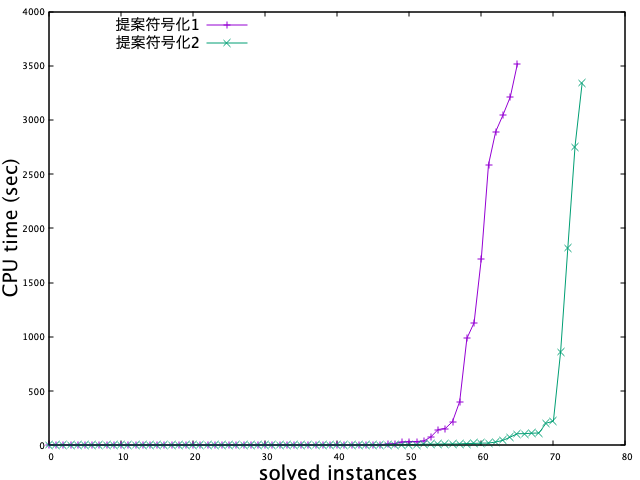
\includegraphics[scale=0.38]{fig/cactus.png}
 \end{figure}

\begin{itemize}
 \item 提案符号化2は,提案符号化1と比較して,より多くの問題を高速に解いている.
\end{itemize}
\end{frame}

%%%%%%%%%%%%%%%%%%%%%%%%%%%%%%%%%%%%%%%%%%%%%%%%%%
%% 辺の数の表
%%%%%%%%%%%%%%%%%%%%%%%%%%%%%%%%%%%%%%%%%%%%%%%%%%
\begin{frame}\frametitle{実験結果(2/2) : 解けた問題数による比較} % 表による比較

\begin{table}[t]
 \centering
 \begin{tabular}{r|c|c|c}
 \hline
 n& h(n)& 圧縮された解の個数& 圧縮率 \\
 \hline
 3&	1&	2&	1.3889 \\
 4&	3&	8&	0.3367 \\
 5&	4&	16&	0.0368 \\
 6&	7&	128&	0.0049 \\
 7&	9&	512&	0.0002 \\
 8&	13&	8192&	- \\
 9&	18&	262144&	- \\
 10&	23&	8388608&	- \\
 11&	29&	536870912&	- \\
 12&	36&	68719476736&	- \\
\end{tabular}
\caption{多色頂点数最大化問題の解の圧縮率}
\label{table:com}
\end{table}

\begin{itemize}
 \item 大規模な問題に対する提案符号化2の有効性が確認できた.
 \item 提案符号化2は,辺の数が40,000を超える問題も解いた.
\end{itemize}

\end{frame}

%%%%%%%%%%%%%%%%%%%%%%%%%%%%%%%%%%%%%%%%%%%%%%%%%%
%% まとめ
%%%%%%%%%%%%%%%%%%%%%%%%%%%%%%%%%%%%%%%%%%%%%%%%%%
\begin{frame}\frametitle{まとめと今後の課題}
 % 自分が伝えたいことをメインに書く
 \begin{block}{まとめ}
  \begin{enumerate}
   \item \structure{根付き全域森問題を解く,2種類のASP符号化を考案した.}
   \begin{itemize}
	\item ASP言語の表現力を用いて,根付き全域森の制約を簡潔に表現できること
		  が確認できた.(ASPのルールで5つ程度)
   \end{itemize}
   \item \structure{実用規模の問題,及び,より大規模な問題を用いた評価実験.}
   \begin{itemize}
	%	\item 提案符号化2は,提案符号化1よりも多くの問題を高速に解いた.
	\item 提案符号化2は,辺の数が40,000を超えるような問題も解くことが
		  でき,大規模な問題に対する有効性が確認できた.
   \end{itemize}
   \item 遷移問題へ拡張し,その符号化を考案した. (本発表では省略)
  \end{enumerate}
 \end{block}
 
 \begin{alertblock}{今後の課題}
  \begin{itemize}
   \item 電気制約への対応.
		 \begin{itemize}
		  \item ASPMT技術を用いた実装.
		 \end{itemize}
   \item 遷移問題へ拡張した符号化の評価実験.
  \end{itemize}
 \end{alertblock}
\end{frame}

%###########################################################
%##### 補助スライド ########################################
%###########################################################
\begin{frame}{~}
 \centering
 - 補足用 -
\end{frame} 

\begin{frame}{補足 : スマートグリッド}
 \begin{itemize}
  \item \structure{スマートグリッド}とは,電力の供給側,需要側において双方向の
		やり取りを可能にする次世代の\structure{賢い}電力網である.
  \item 従来と違い,通信技術の発達により,使用状況などを
		リアルタイムに把握することが可能となった.
  \item その時に応じた最適な配電網を構成し,制御するといったことが考えられている.
		\begin{itemize}
		 \item 電力需要の変化による,配電ロスの少ない構成.
		 \item 自然エネルギーによる発電量の変動を補う構成.
		\end{itemize}
  \item ASP言語の表現力や拡張性が,こうした条件の追加に活用できる可能性がある.
 \end{itemize}
\end{frame}

%%%%%%%%%%%%%%%%%%%%%%%%%%%%%%%%%%%%%%%%%%%%%%%%%%
%% 電気制約
%%%%%%%%%%%%%%%%%%%%%%%%%%%%%%%%%%%%%%%%%%%%%%%%%%
\begin{frame}{補足 : 電気制約}
 \begin{itemize}
  \item \alert{電気制約}は,送電する電流$\cdot$電圧の適正範囲を保証する制約.
  \begin{itemize}
   \item 供給経路の各区間で許容電流を超えない.
   \item 電気抵抗による電圧降下が許容範囲を超えない.
   \item etc.
  \end{itemize}
  \item 電流と電圧が影響し合う\structure{実数ドメイン上の制約}によって表される.
		% \begin{itemize}
		%  		 \item 送電システム上の条件など.
		% \end{itemize}
  \item 実数ドメイン上の制約は,純粋なASPのみで扱うのは\alert{困難}.
		\begin{itemize}
		 \item 緩和問題として,変電所から供給できる家庭の数に上限をつける.
		 \item ASPMT技術により,ASPで得られた解について,
			   背景理論ソルバーと連携して実数ドメイン上の制約を調べる.
		\end{itemize}
 \end{itemize}
\end{frame}


%%%%%%%%%%%%%%%%%%%%%%%%%%%%%%%%%%%%%%%%%%%%%%%%%%
%% 基礎化
%%%%%%%%%%%%%%%%%%%%%%%%%%%%%%%%%%%%%%%%%%%%%%%%%%
\begin{frame}{補足 : ASPシステム}
 
 \vspace{-0.5cm}

 \begin{figure}[htbp]
  \centering
  %%%%%%%%%%%%%%%%%%%%%%%%%%%%%%%%%%%%%%%%%%%%%%%%%%
%% 基礎化の流れの図
%%%%%%%%%%%%%%%%%%%%%%%%%%%%%%%%%%%%%%%%%%%%%%%%%%
\begin{tikzpicture}

 \definecolor{edge}{RGB}{38,38,134}
 \definecolor{node}{RGB}{220,220,249}

 \definecolor{alert_edge}{RGB}{191,0,0}
 \definecolor{alert_node}{RGB}{249,200,200}

 \definecolor{ex_edge}{RGB}{0,96,0}
 \definecolor{ex_node}{RGB}{230,239,230}

 \def\nodespace{2.4cm}

 \tikzset{block/.style={rectangle, thick, draw=edge, fill=node, text width=3cm, 
 text centered, rounded corners, text width=2cm, minimum height=1.5cm}};

 \tikzset{alertblock/.style={rectangle, thick, draw=alert_edge, fill=alert_node, 
 text width=3cm, text centered, rounded corners, text width=1.5cm, minimum height=1.2cm}};

 \node[block](ikkai){一階ASP\\プログラム};

 \node[rectangle,rounded corners, thick, draw=ex_edge, fill=ex_node, 
 right=0.22*\nodespace of ikkai, minimum width=6cm, minimum height=3cm, 
 text centered, label=ASPシステム](sys){};

 \node[block, right=\nodespace of ikkai](meidai){命題ASP\\プログラム};
 \node[block, right=\nodespace of meidai](ASP){解集合};

 \node[right=0.6*\nodespace of ikkai, text width=1.5cm, 
 text centered, text=red, anchor=south](){基礎化\\ソルバー};
 \node[right=0.4*\nodespace of meidai, text width=1.5cm, 
 text centered, text=red, anchor=south](){解集合\\ソルバー};

 
 \foreach \u / \v / \n in {ikkai/meidai,meidai/ASP}
 \draw [thick,->] (\u) to (\v);

\end{tikzpicture}
 \end{figure}

 \vspace{-0.5cm}

 \begin{exampleblock}{}
  \begin{enumerate}
   \item 一階ASPプログラムを基礎化ソルバーによって,
		 命題ASPプログラムに\alert{基礎化}する.
   \item 命題ASPプログラムについて,SAT技術を応用した解集合ソルバーが解集合を探索する.
  \end{enumerate}
 \end{exampleblock}

\end{frame}

%%%%%%%%%%%%%%%%%%%%%%%%%%%%%%%%%%%%%%%%%%%%%%%%%%
%% 遷移問題
%%%%%%%%%%%%%%%%%%%%%%%%%%%%%%%%%%%%%%%%%%%%%%%%%%
\begin{frame}{補足 : 遷移問題}
 \begin{block}{}
   根付き全域森の制約を満たしたまま,各遷移時に変化できる\\
  辺の数は2つ以下として,遷移を求める.
 \end{block}
 \vspace{-0.15cm}
 \begin{exampleblock}{}
  \begin{figure}[htbp]
   \begin{tabular}[tb]{cc}
	\begin{minipage}{0.5\hsize}
	 \centering
	 %%%%%%%%%%%%%%%%%%%%%%%%%%%%%%%%%%%%%%%%%%%%%%%%%%
% 実行例(t=0) (第6章で使う)
%%%%%%%%%%%%%%%%%%%%%%%%%%%%%%%%%%%%%%%%%%%%%%%%%%

\begin{tikzpicture}[x=1.5cm,y=1.5cm,scale=0.7]

 % 設定
 \tikzset{root/.style={circle,draw=black,fill=gray!30,minimum size=1cm}}
 \tikzset{node/.style={circle,draw=black,minimum size=1cm}}
 
 % 補助線
 % \draw [help lines,blue,step=2cm] (-3,0) grid (3,-3);

 % 時間 %
 % \node[rectangle,draw=black] at (-3,1) {$t=0$};

 % root %
 \node[root] at (-2,0) (1){$c_1$};
 \node[above=0.5cm] at (1) {$r_1$};
 \node[root] at (2,0) (3){$c_3$};
 \node[above=0.5cm] at (3) {$r_3$};

 % node %
 \node[node] at (0,0) (2){$c_2$};
 \node[node] at (-2,-2) (4){$c_4$};
 \node[node] at (0,-2) (5){$c_5$};
 \node[node] at (2,-2) (6){$c_6$};

 % 繋がっていない辺は破線
 %\foreach \u / \v in {2/3, 2/5, 4/5}
 %\draw [dashed] (\u) -- (\v);
 % 繋がってる辺は実線
 \foreach \u / \v in {1/2, 1/4, 3/6, 5/6}
 \draw (\u) -- (\v);

 % スイッチ switch %
  \node at (-1,0.2) {$s_1$};
 % \node at (1,0.2) {$s_2$};
  \node at (-2.2,-1) {$s_3$};
 % \node at (-0.2,-1) {$s_4$};
  \node at (1.8,-1) {$s_5$};
 % \node at (-1,-1.8) {$s_6$};
  \node at (1,-1.8) {$s_7$};
 %

\end{tikzpicture}

%%%%%%%%%%%%%%%%%%%%%%%%%%%%%%%%%%%%%%%%%%%%%%%%%%%%%%%%%%
%%% Local Variables:
%%% mode: japanese-latex
%%% TeX-master: paper.tex
%%% End:

	 $t=0$ (初期状態)
	\end{minipage}
	& 
	\hspace{-0.5cm}
	\begin{minipage}{0.5\hsize}
	 \centering
	 %%%%%%%%%%%%%%%%%%%%%%%%%%%%%%%%%%%%%%%%%%%%%%%%%%
% 実行例(t=1) (第6章で使う)
%%%%%%%%%%%%%%%%%%%%%%%%%%%%%%%%%%%%%%%%%%%%%%%%%%

\begin{tikzpicture}[x=1.5cm,y=1.5cm,scale=0.7]

 % 設定
 \tikzset{root/.style={circle,draw=black,fill=gray!30,minimum size=1cm}}
 \tikzset{node/.style={circle,draw=black,minimum size=1cm}}
 
 % 補助線
 % \draw [help lines,blue,step=2cm] (-3,0) grid (3,-3);

 % 時間 %
 % \node[rectangle,draw=black] at (-3,1) {$t=1$};

 % root %
 \node[root] at (-2,0) (1){$c_1$};
 \node[above=0.5cm] at (1) {$r_1$};
 \node[root] at (2,0) (3){$c_3$};
 \node[above=0.5cm] at (3) {$r_3$};

 % node %
 \node[node] at (0,0) (2){$c_2$};
 \node[node] at (-2,-2) (4){$c_4$};
 \node[node] at (0,-2) (5){$c_5$};
 \node[node] at (2,-2) (6){$c_6$};

 % 繋がっていない辺は破線
 %\foreach \u / \v in {2/3, 2/5, 4/5}
 %\draw [dashed] (\u) -- (\v);
 % 繋がってる辺は実線
 \foreach \u / \v in {2/3, 1/4, 3/6, 5/6}
 \draw (\u) -- (\v);

 % スイッチ switch %
 % \node at (-1,0.2) {$s_1$};
 %
 \node at (1,0.2) {$s_2$};
 \node at (-2.2,-1) {$s_3$};
 % \node at (-0.2,-1) {$s_4$};
 \node at (1.8,-1) {$s_5$};
 % \node at (-1,-1.8) {$s_6$};
 \node at (1,-1.8) {$s_7$};
 %

\end{tikzpicture}

%%%%%%%%%%%%%%%%%%%%%%%%%%%%%%%%%%%%%%%%%%%%%%%%%%%%%%%%%%
%%% Local Variables:
%%% mode: japanese-latex
%%% TeX-master: paper.tex
%%% End:

	 $t=1$
	\end{minipage} 
   \end{tabular}\\
   \vspace{0.25cm}
   \begin{tabular}[tb]{cc}
	\begin{minipage}{0.5\hsize}
	 \centering
	 %%%%%%%%%%%%%%%%%%%%%%%%%%%%%%%%%%%%%%%%%%%%%%%%%%
% 実行例(t=2) (第6章で使う)
%%%%%%%%%%%%%%%%%%%%%%%%%%%%%%%%%%%%%%%%%%%%%%%%%%

\begin{tikzpicture}[x=1.5cm,y=1.5cm,scale=0.7]

 % 設定
 \tikzset{root/.style={circle,draw=black,fill=gray!30,minimum size=1cm}}
 \tikzset{node/.style={circle,draw=black,minimum size=1cm}}
 
 % 補助線
 % \draw [help lines,blue,step=2cm] (-3,0) grid (3,-3);

 % 時間 %
 % \node[rectangle,draw=black] at (-3,1) {$t=2$};

 % root %
 \node[root] at (-2,0) (1){$1$};
% \node[above=0.5cm] at (1) {$r_1$};
 \node[root] at (2,0) (3){$3$};
 %\node[above=0.5cm] at (3) {$r_3$};

 % node %
 \node[node] at (0,0) (2){$2$};
 \node[node] at (-2,-2) (4){$4$};
 \node[node] at (0,-2) (5){$5$};
 \node[node] at (2,-2) (6){$6$};

 % 繋がっていない辺は破線
 %\foreach \u / \v in {2/3, 2/5, 4/5}
 %\draw [dashed] (\u) -- (\v);
 % 繋がってる辺は実線
 \foreach \u / \v in {2/3, 4/5, 3/6, 5/6}
 \draw (\u) -- (\v);

 % スイッチ switch %
 % \node at (-1,0.2) {$s_1$};
 % \node at (1,0.2) {$s_2$};
 % \node at (-2.2,-1) {$s_3$};
 % \node at (-0.2,-1) {$s_4$};
 % \node at (1.8,-1) {$s_5$};
 % \node at (-1,-1.8) {$s_6$};
 % \node at (1,-1.8) {$s_7$};
 %

\end{tikzpicture}

%%%%%%%%%%%%%%%%%%%%%%%%%%%%%%%%%%%%%%%%%%%%%%%%%%%%%%%%%%
%%% Local Variables:
%%% mode: japanese-latex
%%% TeX-master: paper.tex
%%% End:

	 $t=2$
	\end{minipage}
	&
	\hspace{-0.5cm}
	\begin{minipage}{0.5\hsize}
	\centering
	 %%%%%%%%%%%%%%%%%%%%%%%%%%%%%%%%%%%%%%%%%%%%%%%%%%
% 実行例(t=3) (第6章で使う)
%%%%%%%%%%%%%%%%%%%%%%%%%%%%%%%%%%%%%%%%%%%%%%%%%%
\begin{tikzpicture}[scale=0.6]

 % 設定
 \tikzset{node/.style={circle,draw=black,fill=white}}

 \definecolor{edge1}{RGB}{191,0,0}
 \definecolor{node1}{RGB}{249,200,200}
 \definecolor{edge3}{RGB}{38,38,134}
 \definecolor{node3}{RGB}{200,200,249}

 % 補助線
 % \draw [help lines,blue] (0,0) grid (20,6);

 % node %
 \node[circle, ultra thick, draw=edge1, fill=node1](out1){1};
 \node[node, fill=node3, right=of out1] (out2){2};
 \node[circle, ultra thick, draw=edge3,fill=node3, right=of out2](out3){3};
 \node[node, fill=node3, below=of out1] (out4){4};
 \node[node, fill=node3, below=of out2] (out5){5};
 \node[node, fill=node3, below=of out3] (out6){6};

 \foreach \u / \v in {}
 \draw [very thick, edge1] (\u) -- (\v);

 \foreach \u / \v in {out2/out3,out2/out5,out4/out5,out5/out6}
 \draw [very thick, edge3](\u) -- (\v);
\end{tikzpicture}

%%%%%%%%%%%%%%%%%%%%%%%%%%%%%%%%%%%%%%%%%%%%%%%%%%%%%%%%%%
%%% Local Variables:
%%% mode: japanese-latex
%%% TeX-master: paper.tex
%%% End:

	 $t=3$ (目的状態)
	\end{minipage}
   \end{tabular}
  \end{figure}
 \end{exampleblock}
\end{frame}


%%%%%%%%%%%%%%%%%%%%%%%%%%%%%%%%%%%%%%%%%%%%%%%%%%
%% ASPのコード
%%%%%%%%%%%%%%%%%%%%%%%%%%%%%%%%%%%%%%%%%%%%%%%%%%
\begin{frame}[fragile]{補足 : 提案符号化1のASPプログラム}
 \begin{exampleblock}{}
  \begin{center}
   %%%%%%%%%%%%%%%%%%%%%%%%%%%%%%%%%
   \lstinputlisting[numbers=left,%
   basicstyle=\ttfamily\tiny]{code/srf1.lp}
   %%%%%%%%%%%%%%%%%%%%%%%%%%%%%%%%% 
  \end{center}
 \end{exampleblock}
\end{frame}

\begin{frame}[fragile]{補足 : 提案符号化2のASPプログラム}

 \begin{exampleblock}{}
  \begin{center}
   %%%%%%%%%%%%%%%%%%%%%%%%%%%%%%%%%
   \lstinputlisting[numbers=left,%
   basicstyle=\ttfamily\tiny]{code/srf2.lp}
   %%%%%%%%%%%%%%%%%%%%%%%%%%%%%%%%% 
  \end{center}
 \end{exampleblock}

\end{frame}


\end{document}